\newpage
\section{Giao diện người dùng và quản trị hệ thống}

Giao diện người dùng của trục tích hợp dữ liệu được thiết kế dưới dạng một trang quản trị tập trung, cung cấp cho quản trị viên khả năng giám sát, điều khiển và bảo vệ luồng dữ liệu của toàn bộ hệ thống. Giao diện được chia thành ba phân hệ chính, tương ứng với các nghiệp vụ cốt lõi: bảng điều khiển trung tâm, quản lý lịch sử đồng bộ và quản lý sao lưu dữ liệu.

\subsection{Bảng điều khiển trung tâm}

Bảng điều khiển trung tâm là nơi cung cấp cái nhìn tổng quan nhất về trạng thái hoạt động của trục tích hợp theo thời gian thực. Phân hệ này được thiết kế với bốn thành phần chức năng chính:

\begin{enumerate}
    \item \textbf{Kích hoạt đồng bộ thủ công:} Quản trị viên có thể kích hoạt tiến trình đồng bộ ngay lập tức. Hệ thống hỗ trợ hai chế độ: đồng bộ toàn phần hoặc đồng bộ tùy chỉnh (chỉ chọn một số bảng dữ liệu cụ thể thông qua hộp thoại lựa chọn). Trong quá trình xử lý, nút kích hoạt sẽ bị vô hiệu hóa tạm thời để tránh việc gọi hàm lặp lại.
    
    \item \textbf{Quản lý tác vụ định kỳ:} Hệ thống cung cấp giao diện để tạo mới, bật/tắt và cập nhật các tác vụ tự động dựa trên biểu thức Cron. Với mỗi tác vụ, hệ thống hiển thị rõ ràng thông tin về thời gian thực thi gần nhất và thời gian dự kiến cho lần chạy tiếp theo.
    
    \item \textbf{Thống kê chỉ số thực thi:} Sử dụng biểu đồ cột để trực quan hóa số lượng bản ghi đồng bộ thành công và thất bại trong bảy lần chạy gần nhất. Chức năng này giúp quản trị viên dễ dàng nhận biết xu hướng và phát hiện các dấu hiệu bất thường của hệ thống.
    
    \item \textbf{Cửa sổ giám sát thời gian thực:} Đây là một điểm nhấn kỹ thuật của giao diện. Hệ thống thiết lập một kết nối liên tục đến máy chủ thông qua công nghệ Server-Sent Events (SSE). Nhờ đó, mọi nhật ký hoạt động từ máy chủ đều được đẩy trực tiếp lên giao diện và tự động cuộn xuống dòng mới nhất, giúp quản trị viên theo dõi sát sao từng bước của tiến trình ETL mà không cần làm mới trang.
\end{enumerate}

\begin{figure}
    \centering
    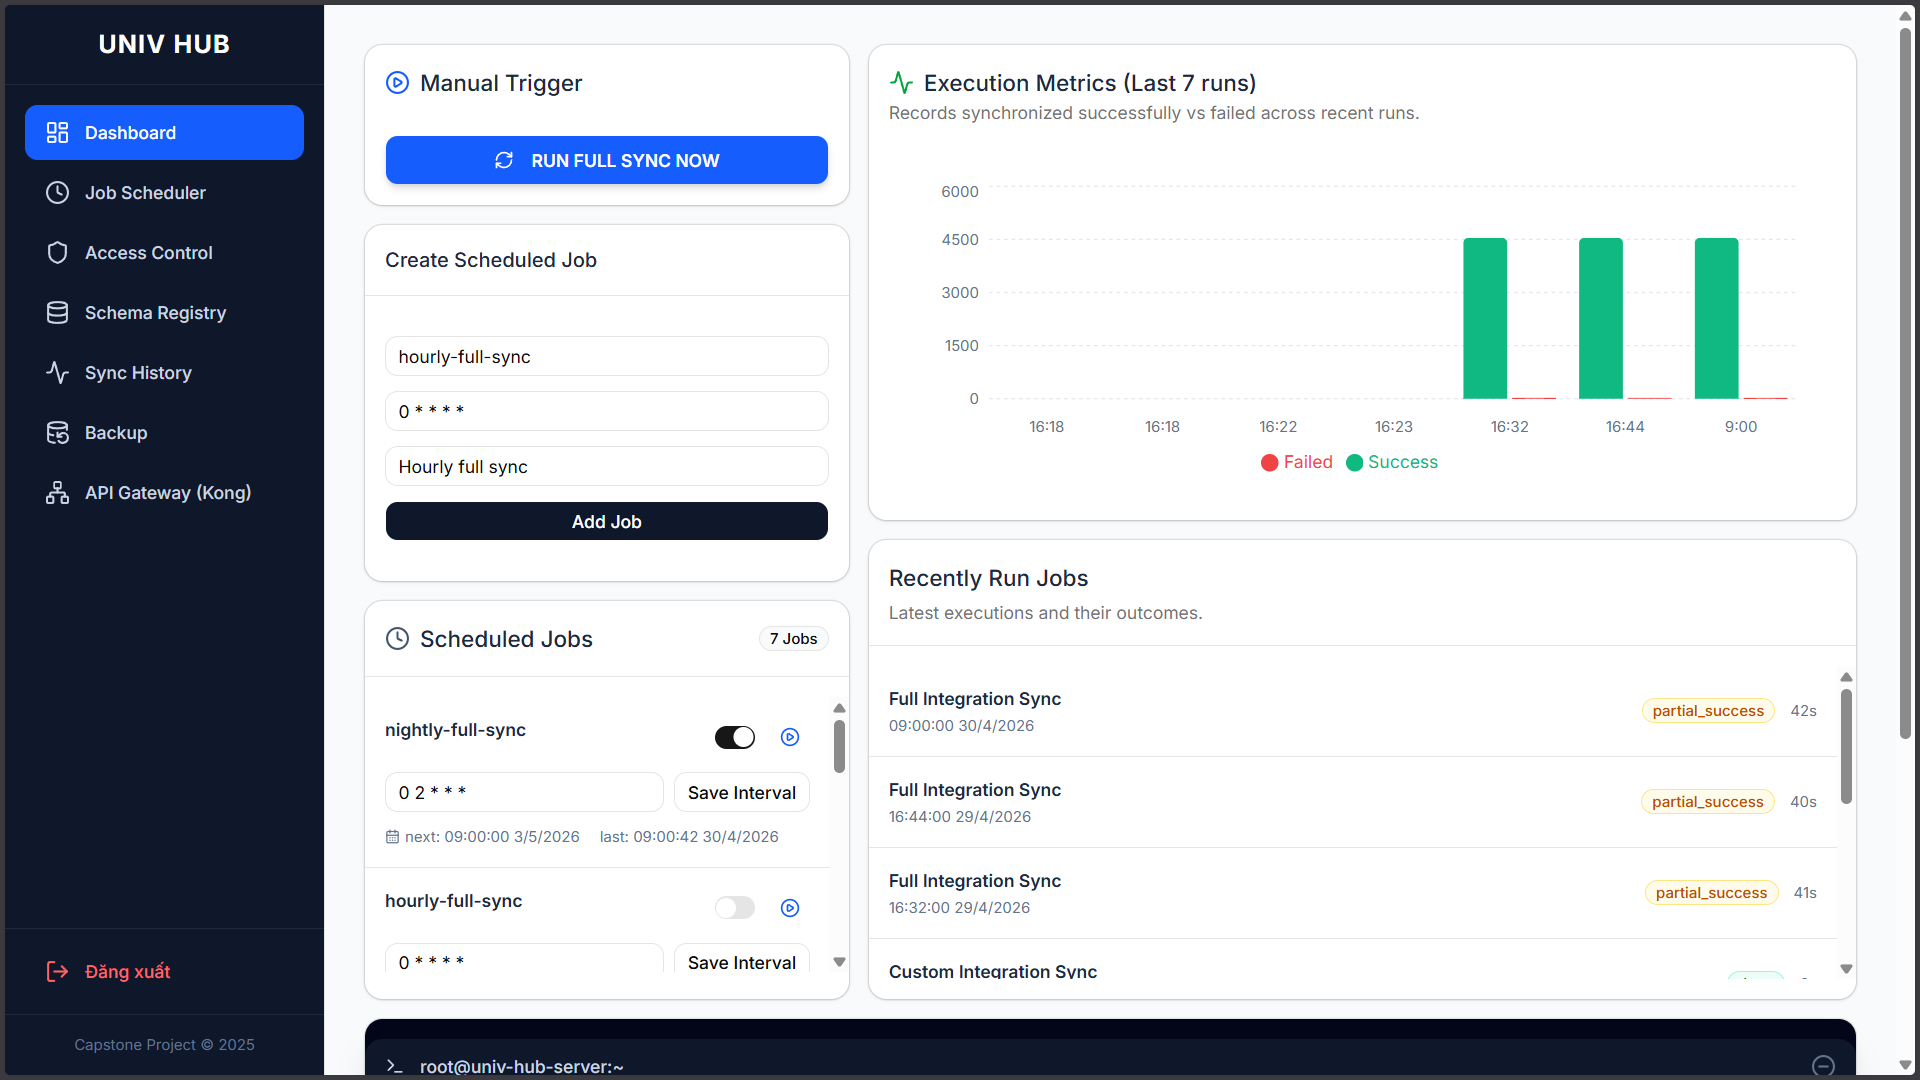
\includegraphics[width=1\linewidth]{graphics/dashboard.png}
    \caption{Giao diện bảng điều khiển trung tâm}
    \label{fig:dashboard-ui}
\end{figure}

\subsection{Quản lý lịch sử đồng bộ}

Do tính chất phức tạp của việc tích hợp nhiều nguồn dữ liệu khác nhau, phân hệ quản lý lịch sử đồng bộ được thiết kế theo mô hình phân cấp chính - phụ nhằm tối ưu hóa không gian hiển thị:

\begin{itemize}
    \item \textbf{Mức tiến trình:} Hiển thị danh sách các lần thực thi, bao gồm thông tin về tên tiến trình, thời gian bắt đầu, tổng thời lượng thực thi, trạng thái tổng thể (thành công, đang chạy, lỗi một phần, thất bại) và tổng số lượng bản ghi được xử lý.
    
    \item \textbf{Mức bảng dữ liệu:} Khi mở rộng một dòng tiến trình, giao diện sẽ hiển thị chi tiết kết quả đồng bộ của từng bảng dữ liệu riêng biệt. Quản trị viên có thể biết chính xác bảng nào được cập nhật bao nhiêu bản ghi, bảng nào bị bỏ qua hoặc bảng nào gặp lỗi.
    
    \item \textbf{Truy xuất nhật ký lỗi nguyên bản:} Đối với các bản ghi hoặc bảng dữ liệu gặp sự cố, quản trị viên có thể mở hộp thoại xem chi tiết lỗi hệ thống. Hệ thống trích xuất và hiển thị thông báo lỗi gốc từ bộ phân tích hoặc cơ sở dữ liệu, hỗ trợ tối đa cho quá trình gỡ lỗi.
\end{itemize}

\begin{figure}
    \centering
    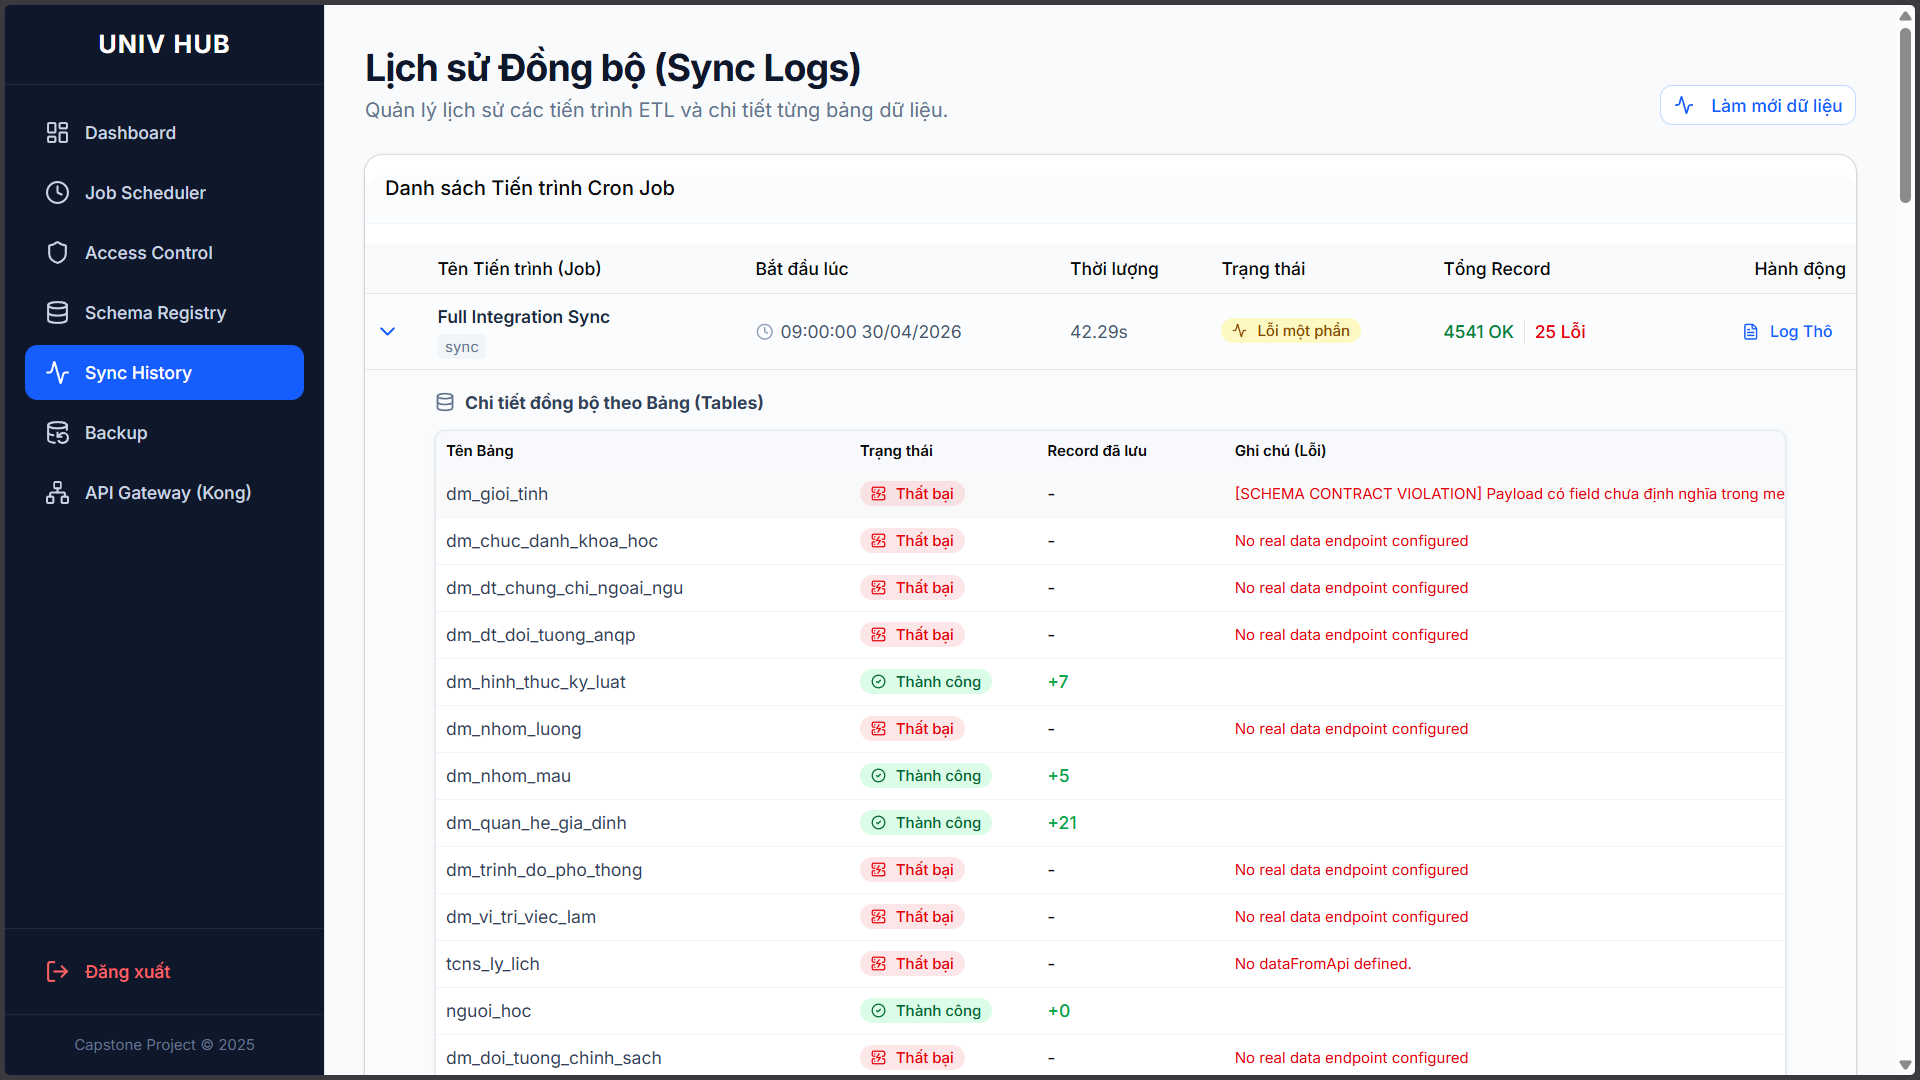
\includegraphics[width=1\linewidth]{graphics/sync-ui.png}
    \caption{Giao diện quản lý lịch sử đồng bộ}
    \label{fig:sync-ui}
\end{figure}

\subsection{Quản lý sao lưu và phục hồi}

An toàn dữ liệu là yếu tố kiên quyết trong trục tích hợp. Phân hệ quản lý sao lưu cung cấp các công cụ tương tác trực tiếp với hệ thống lưu trữ tập tin. Giao diện phân loại các tệp sao lưu thành bốn nhóm tương ứng với ngữ cảnh tạo ra chúng:

\begin{enumerate}
    \item \textbf{Sao lưu thủ công:} Các bản sao lưu do quản trị viên chủ động tạo ra thông qua giao diện.
    \item \textbf{Sao lưu định kỳ:} Các bản sao lưu được tạo bởi hệ thống theo lịch trình tự động.
    \item \textbf{Trước đồng bộ:} Các bản chụp trạng thái dữ liệu được hệ thống tự động tạo ra ngay trước khi tiến hành ghi đè dữ liệu mới từ nguồn.
    \item \textbf{Lược đồ thay đổi:} Các bản sao lưu được tạo ra khi hệ thống phát hiện có sự thay đổi về cấu trúc bảng từ nguồn.
\end{enumerate}

Quy trình quản lý sao lưu được thiết kế theo luồng hai bước để tránh làm rối giao diện. Ở bước đầu tiên, hệ thống liệt kê danh sách các bảng dữ liệu hiện có bản sao lưu. Khi quản trị viên chọn một bảng cụ thể, hệ thống mới hiển thị danh sách chi tiết các tệp sao lưu của bảng đó theo mốc thời gian. 

Tại đây, quản trị viên có thể tải tệp sao lưu trực tiếp về máy tính cá nhân thông qua cơ chế URL định tuyến an toàn hoặc nhấn nút phục hồi dữ liệu. Để đảm bảo an toàn, mọi thao tác phục hồi đều yêu cầu một bước xác nhận cảnh báo từ người dùng nhằm tránh việc ghi đè dữ liệu hiện tại do sơ suất.

\begin{figure}
    \centering
    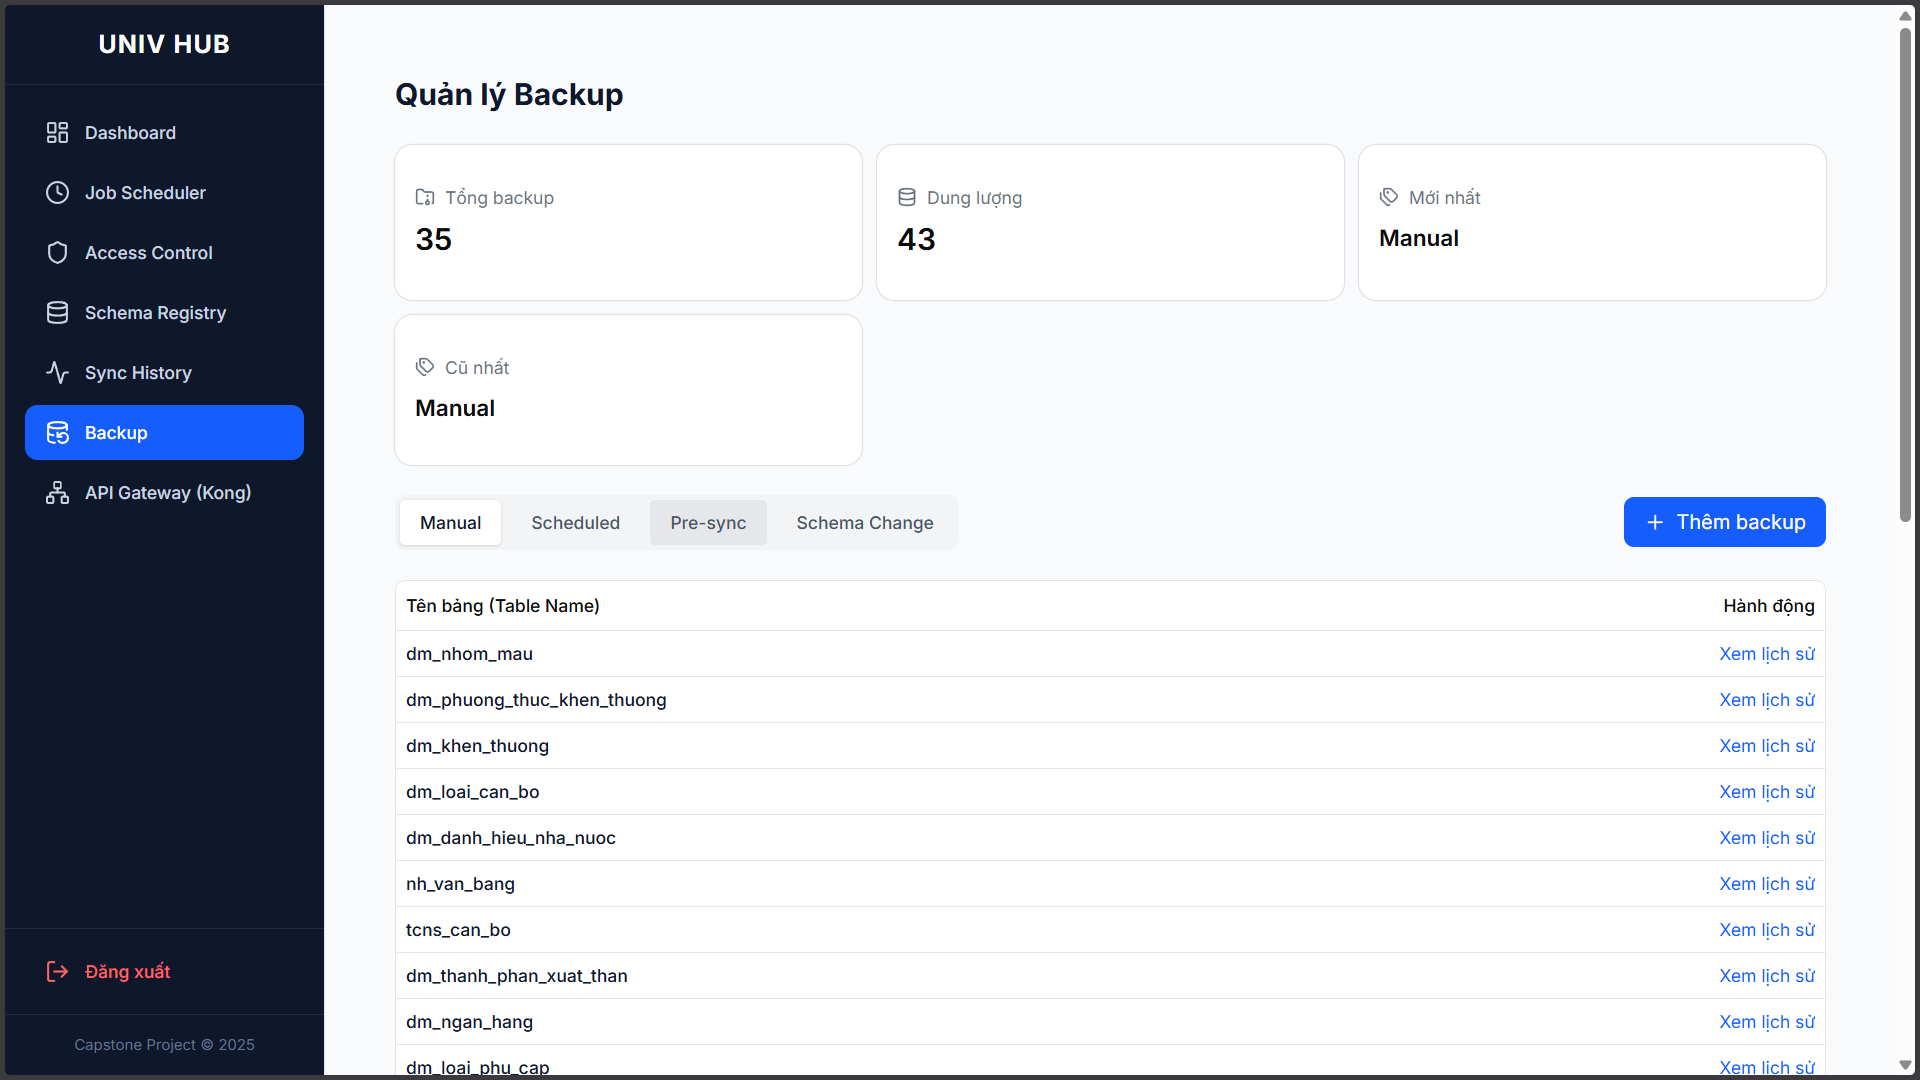
\includegraphics[width=1\linewidth]{graphics/backup-ui.png}
    \caption{Giao diện quản lý sao lưu và phục hồi dữ liệu}
    \label{fig:backup-ui}
\end{figure}

\subsection{Quản lý phân quyền truy cập}

Để đảm bảo tính bảo mật và ngăn chặn việc lạm dụng quyền hạn trong thao tác với dữ liệu, trục tích hợp cung cấp một phân hệ quản lý phân quyền dựa trên vai trò người dùng. Thông qua giao diện này, quản trị viên cấp cao có thể dễ dàng kiểm soát và giới hạn phạm vi truy cập đối với từng cá nhân hoặc hệ thống bên thứ ba khi họ tương tác với dữ liệu trên trục tích hợp.

Giao diện quản lý phân quyền bao gồm một bảng tổng hợp danh sách người dùng, hiển thị trực quan vai trò hiện tại (như quản trị viên, người dùng đọc, người dùng ghi) và các quyền hạn cụ thể đã được cấp phát. 

Khi cần thay đổi quyền hạn, quản trị viên có thể mở bảng điều khiển chỉnh sửa bên cạnh (side-panel). Tại đây, ngoài việc thay đổi vai trò tổng thể, hệ thống còn cho phép thiết lập các quyền truy cập chi tiết đến từng bảng dữ liệu (Scope) thông qua cơ chế biểu thức chính quy (Regular Expression). Cụ thể:
\begin{itemize}
    \item \textbf{Phạm vi đọc:} Danh sách các bảng dữ liệu mà tài khoản được phép truy vấn. (Ví dụ: thiết lập \texttt{\^dm\_.*} cho phép người dùng đọc tất cả các bảng danh mục).
    \item \textbf{Phạm vi ghi:} Danh sách các bảng dữ liệu mà tài khoản được phép chèn, cập nhật hoặc xóa (chỉ áp dụng đối với những người dùng được cấp vai trò cho phép thao tác ghi).
\end{itemize}

Cơ chế phân quyền này giúp phân tách rõ ràng ranh giới dữ liệu giữa các phòng ban, đảm bảo phòng ban nào chỉ được xem và xử lý đúng phần dữ liệu thuộc thẩm quyền của mình.

\begin{figure}
    \centering
    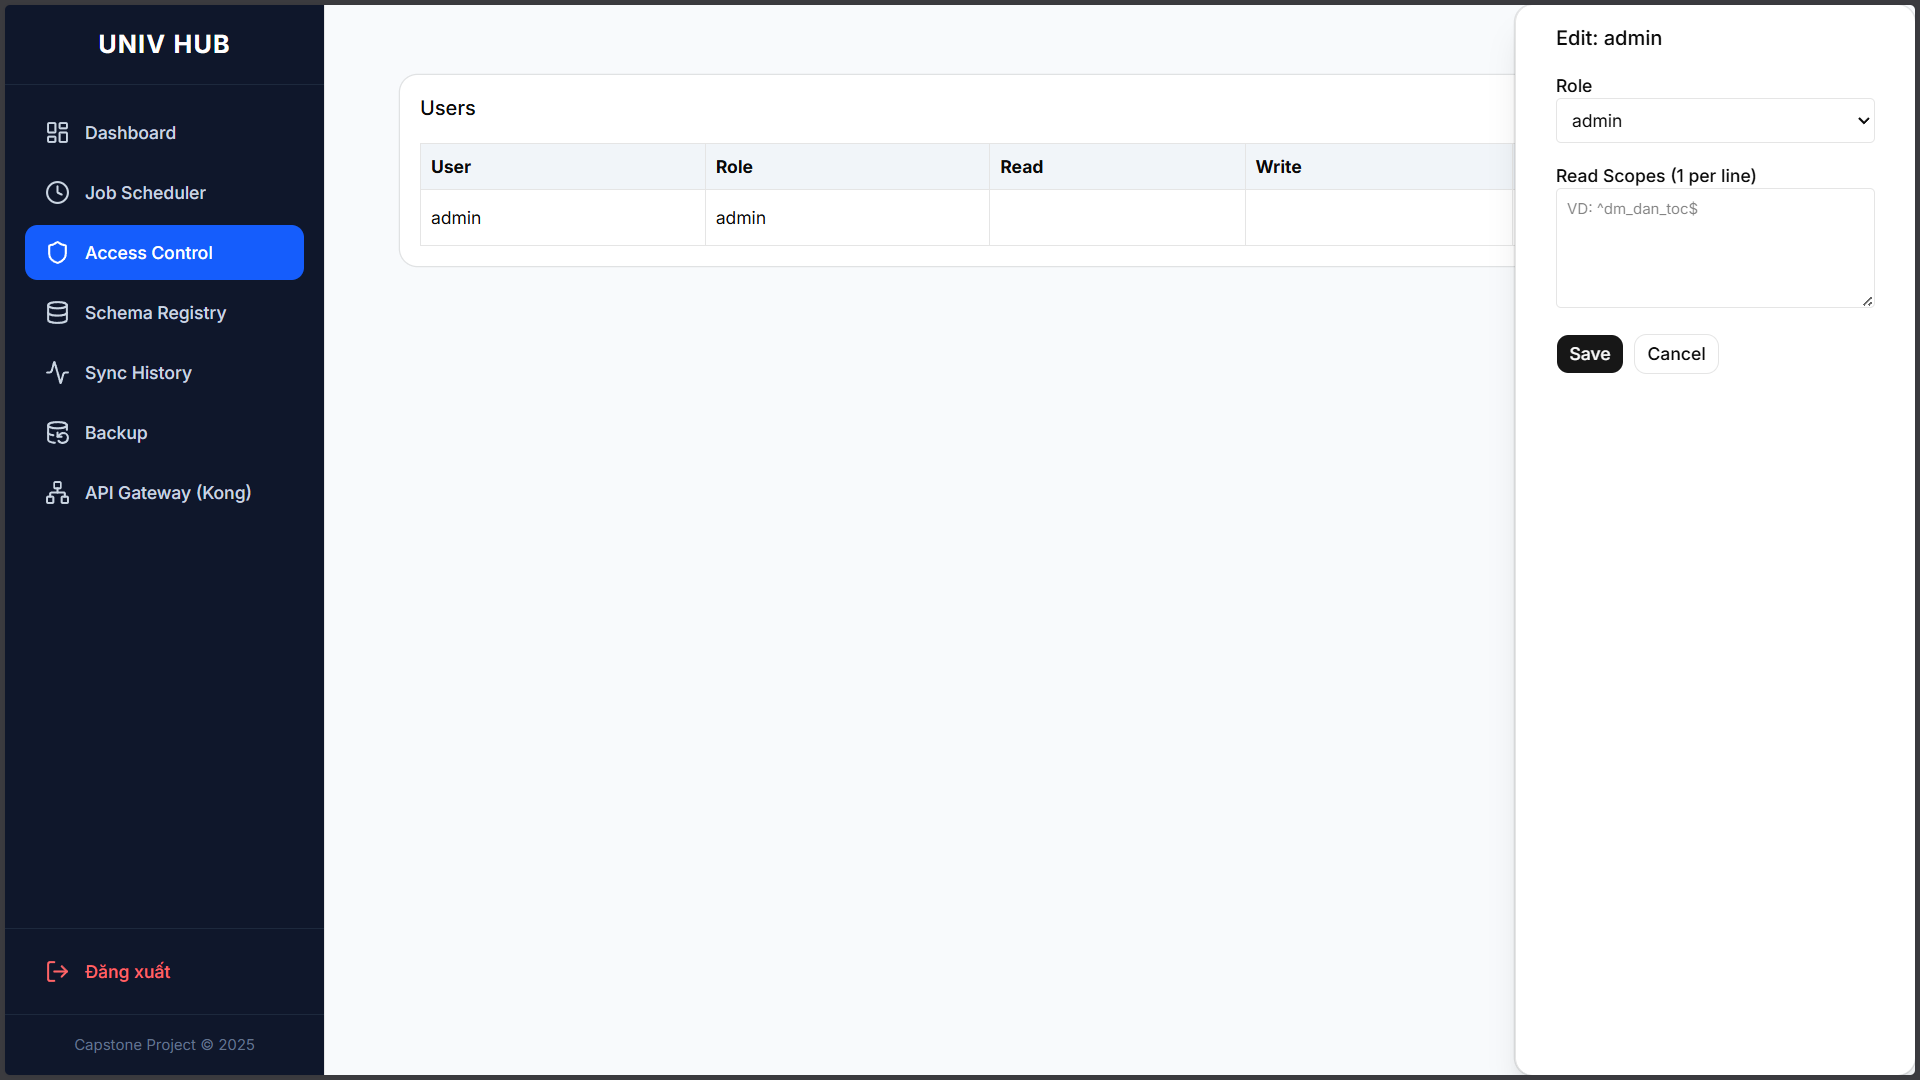
\includegraphics[width=1\linewidth]{graphics/access-control.png}
    \caption{Giao diện quản lý phân quyền truy cập cho người dùng}
    \label{fig:access-control}
\end{figure}

\subsection{Quản lý và đối soát lược đồ dữ liệu}

Trong kiến trúc tích hợp dữ liệu phân tán, việc các hệ thống nguồn tự ý thay đổi cấu trúc bảng (thêm, sửa, xóa cột) mà không thông báo trước là một trong những nguyên nhân hàng đầu gây sụp đổ luồng dữ liệu. Để giải quyết rủi ro này, hệ thống cung cấp một phân hệ quản lý và đối soát lược đồ dữ liệu chuyên sâu.

Giao diện hiển thị danh sách tất cả các bảng dữ liệu mà trục tích hợp đang theo dõi, kèm theo trạng thái ổn định của từng bảng. Nếu hệ thống nguồn có sự thay đổi về cấu trúc trả về, trạng thái của bảng sẽ lập tức chuyển sang cảnh báo thay đổi (\textit{Schema Drift}), đồng thời mọi tiến trình đồng bộ dữ liệu vào bảng này sẽ tự động bị đình chỉ tạm thời để bảo vệ cơ sở dữ liệu đích.

Hộp thoại so sánh lược đồ dữ liệu được lấy cảm hứng từ GithHub. Khi quản trị viên chọn xem xét một bảng đang bị cảnh báo, hệ thống sẽ thực hiện các thuật toán tính toán và hiển thị trực quan sự khác biệt:
\begin{itemize}
    \item \textbf{So sánh song song:} Giao diện chia thành hai cột, một bên là cấu trúc mới vừa nhận được từ nguồn, bên còn lại là cấu trúc cũ đang được lưu trữ trong cơ sở dữ liệu.
    \item \textbf{Phân loại thay đổi:} Các trường dữ liệu được đánh dấu màu sắc rõ ràng tương ứng với ba trạng thái: mới được thêm vào, đã bị thay đổi (như đổi kiểu dữ liệu hoặc độ dài) và đã bị xóa bỏ.
    \item \textbf{Cảnh báo rủi ro cao:} Nếu hệ thống phát hiện có trường dữ liệu bị xóa hoặc thay đổi kiểu (có nguy cơ gây mất dữ liệu hiện có), một thông báo cảnh báo màu đỏ sẽ xuất hiện, yêu cầu quản trị viên hết sức cẩn trọng.
\end{itemize}

Hơn thế nữa, để tự động hóa tối đa quy trình cập nhật, giao diện còn tích hợp tính năng tự động sinh mã nguồn (Auto-generate Code). Hệ thống sẽ chuyển đổi các kiểu dữ liệu từ cấu trúc của hệ thống nguồn sang định dạng chuẩn của Prisma ORM và tạo sẵn đoạn mã khai báo mô hình dữ liệu (Prisma Model). Quản trị viên chỉ cần nhấn nút sao chép, dán vào mã nguồn của trục tích hợp và chạy lệnh đồng bộ cơ sở dữ liệu mà không cần phải tự viết tay lại từ đầu. 

Sau khi quá trình cập nhật cấu trúc cơ sở dữ liệu hoàn tất một cách an toàn, quản trị viên sẽ nhấn nút xác nhận trên giao diện. Lúc này, trạng thái của bảng sẽ trở lại trạng thái ổn định và các luồng đồng bộ dữ liệu sẽ tự động hoạt động trở lại bình thường.

\begin{figure}[H]
    \centering
    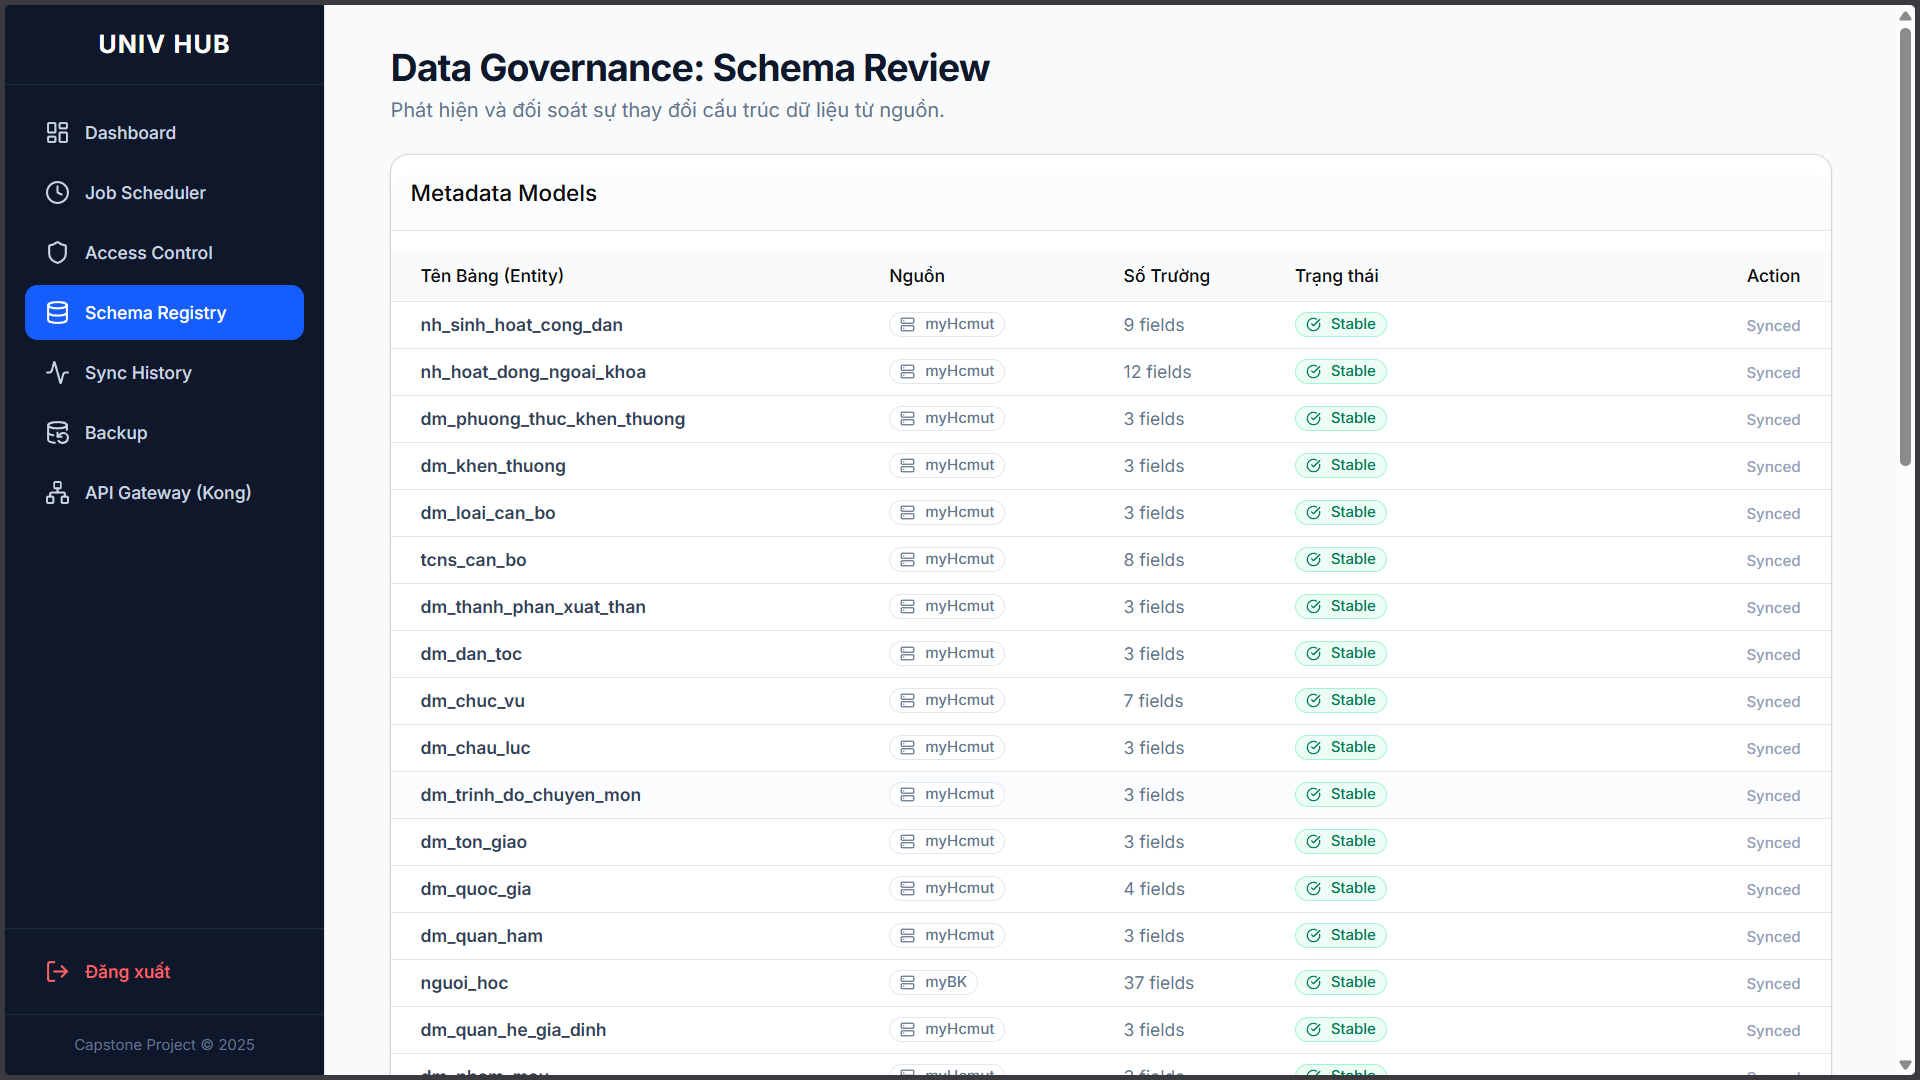
\includegraphics[width=1\linewidth]{graphics/schema.png}
    \caption{Giao diện quản lý lược đồ dữ liệu}
    \label{fig:schema-ui}
\end{figure}